\documentclass[12pt]{article}

\usepackage{amsmath}
\usepackage{array}
\usepackage{caption}
\usepackage[top=1in, bottom=1in, left=0.75in, right=0.75in]{geometry}

\usepackage{graphicx}
\graphicspath{{figures/}}

\usepackage[colorlinks=true, allcolors=blue]{hyperref}
\usepackage[utf8]{inputenc}
\usepackage{multirow}
\usepackage{pdfpages}
\usepackage[section]{placeins}


\begin{document}

\begin{titlepage}
  \begin{center} \LARGE
    \vspace*{1.5in}

    ECE 272 Pre-Lab 6

    Fall 2018

    \vfill

    Video Graphics Array (VGA)

    Phi Luu

    \vfill

    November 14\textsuperscript{th}, 2018

    Grading TA: Edgar Perez

    \vspace{1.5in}
  \end{center}
\end{titlepage}

\begin{enumerate}
  \item Read everything you can about VGA
  \item Create a block diagram and write about how it works.

  A video graphics array (VGA) connector is a three-row 15-pin connector that carries analog component RGBHV (red, green, blue, horizontal sync, vertical sync) video signals and VESA display data channel (VESA DDC) data. The pinout of a VGA female socket is illustrated by Figure~\ref{fig:vga_female_socket} below:

  \begin{figure}[ht]
    \centering
    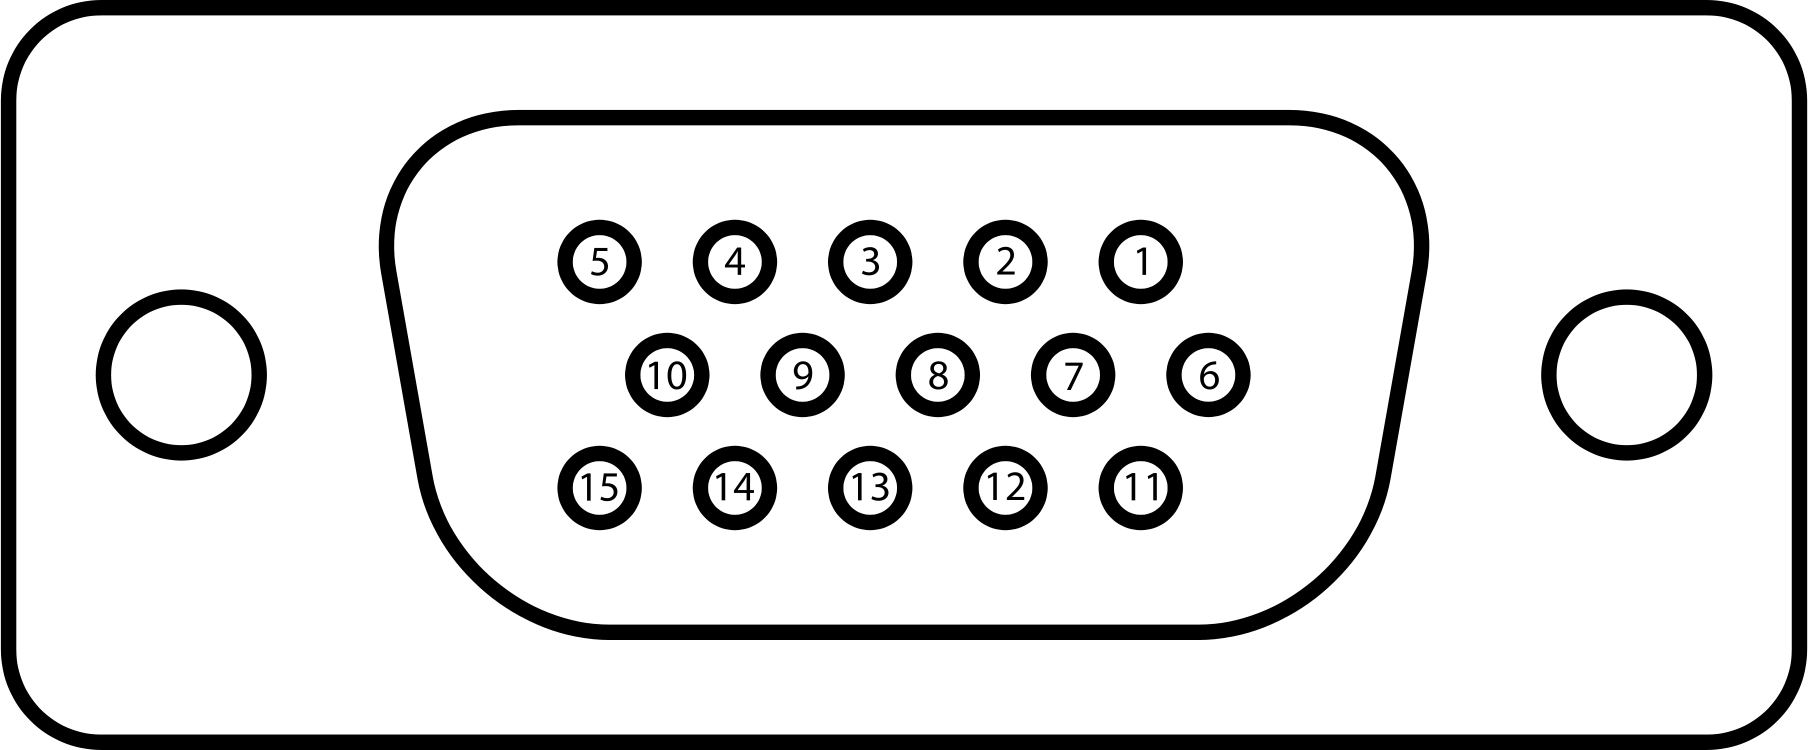
\includegraphics[width=0.5\textwidth]{vga_female_socket.png}
    \caption{A female VGA socket}
    \label{fig:vga_female_socket}
  \end{figure}

  The pin layout of this socket is explained in Table~\ref{tab:vga_pin_layout}

  \begin{table}[ht]
    \centering
    \begin{tabular}{ | c | c | l | }
    \hline
    \textbf{Pin} & \textbf{Signal} & \textbf{Description}                                                                     \\ \hline
    1            & RED             & Red video                                                                                \\ \hline
    2            & GREEN           & Green video                                                                              \\ \hline
    3            & BLUE            & Blue video                                                                               \\ \hline
    4            & ID2/RES         & \begin{tabular}[c]{@{}l@{}}formerly Monitor ID bit 2\\ Reserved since E-DDC\end{tabular} \\ \hline
    5            & GND             & Ground (H-Sync)                                                                          \\ \hline
    6            & RED\_RTN        & Red return                                                                               \\ \hline
    7            & GREEN\_RTN      & Green return                                                                             \\ \hline
    8            & BLUE\_RTN       & Blue return                                                                              \\ \hline
    9            & KEY/PWR         & \begin{tabular}[c]{@{}l@{}}formerly key\\ now +5V DC\end{tabular}                        \\ \hline
    10           & GND             & Ground (V-Sync, DDC)                                                                     \\ \hline
    11           & ID0/RES         & \begin{tabular}[c]{@{}l@{}}formerly Monitor ID bit 0\\ reserved since E-DDC\end{tabular} \\ \hline
    12           & ID1/SDA         & \begin{tabular}[c]{@{}l@{}}formerly Monitor ID bit 1\\ PC data since DDC2\end{tabular}   \\ \hline
    13           & HSync           & Horizontal sync                                                                          \\ \hline
    14           & VSync           & Vertical sync                                                                            \\ \hline
    15           & ID3/SCL         & \begin{tabular}[c]{@{}l@{}}formerly Monitor ID bit 3\\ I2C clock since DDC2\end{tabular} \\ \hline
    \end{tabular}
    \caption{VGA pin layout}
    \label{tab:vga_pin_layout}
  \end{table}

  Using the red, green, blue, hsync, and vsync signals, the VGA can encode these color into information to transfer to a display device which essentially displays the specified graphics to the real world.

  For each line of the screen, there is an empty line where no graphics are displayed, allowing the "cursor" to move back from the right edge to the left edge of the screen and get ready for displaying the next line of graphics.
\end{enumerate}

\end{document}
